% SPDX-License-Identifier: CC-BY-4.0
% Psi-treillis: the article. Every number comes from numbers.tex, which tools/paper_numbers.py writes from the logs of
% benchmarks/. Build: see README.md in this folder.
\documentclass[11pt,a4paper]{article}
\usepackage[T1]{fontenc}
\usepackage[utf8]{inputenc}
\usepackage{lmodern}
\usepackage[margin=2.5cm]{geometry}
\usepackage{amsmath,amssymb}
\usepackage{graphicx}
\usepackage{booktabs}
\usepackage{microtype}
\usepackage{xcolor}
\usepackage[numbers,sort&compress]{natbib}
\usepackage[hidelinks]{hyperref}
\hypersetup{pdftitle={Psi-treillis: divergence-free compression of periodic turbulent velocity fields, sampled on the GPU without rebuilding the grid},
            pdfauthor={Killian Pluenet}}
\usepackage{xurl}
\usepackage{caption}
\usepackage{longtable}
\usepackage{tikz}
\usetikzlibrary{arrows.meta,positioning}
\captionsetup{font=small,labelfont=bf}

% Written by tools/paper_numbers.py from the logs of benchmarks/. Do not edit: run the script again.
\expandafter\def\csname val@claims.fail\endcsname{10}
\expandafter\def\csname val@claims.hold\endcsname{28}
\expandafter\def\csname val@claims.pending\endcsname{9}
\expandafter\def\csname val@claims.total\endcsname{47}
\expandafter\def\csname val@comp.256.d3.t03.ratio\endcsname{105.1}
\expandafter\def\csname val@comp.256.d3.t04.ratio\endcsname{127.3}
\expandafter\def\csname val@comp.256.d3.t05.ratio\endcsname{134.1}
\expandafter\def\csname val@comp.512.d2.ratio\endcsname{119}
\expandafter\def\csname val@comp.512.d2.rms\endcsname{0.69}
\expandafter\def\csname val@comp.512.d3.ratio\endcsname{143}
\expandafter\def\csname val@comp.512.d3.rms\endcsname{0.64}
\expandafter\def\csname val@comp.512.d3.t03.ratio\endcsname{100.1}
\expandafter\def\csname val@comp.512.d3.t04.ratio\endcsname{126.5}
\expandafter\def\csname val@comp.512.d3.t05.ratio\endcsname{136.6}
\expandafter\def\csname val@ctrl.ratio.max\endcsname{1.09}
\expandafter\def\csname val@ctrl.ratio.min\endcsname{1.06}
\expandafter\def\csname val@div.psi.max\endcsname{$9.4\times10^{-16}$}
\expandafter\def\csname val@enc.512.t03\endcsname{435}
\expandafter\def\csname val@enc.512.t05\endcsname{275}
\expandafter\def\csname val@eq.256.other.points\endcsname{20}
\expandafter\def\csname val@eq.256.psi.rms.max\endcsname{0.61}
\expandafter\def\csname val@eq.256.psi.rms.min\endcsname{0.58}
\expandafter\def\csname val@eq.256.psi.t05.ratio\endcsname{134}
\expandafter\def\csname val@eq.256.psi.t05.rms\endcsname{0.61}
\expandafter\def\csname val@eq.256.sz4d.over.psi.max\endcsname{2.5}
\expandafter\def\csname val@eq.256.sz4d.over.psi.min\endcsname{1.9}
\expandafter\def\csname val@eq.256.sz4d.rms.over.psi.max\endcsname{2.8}
\expandafter\def\csname val@eq.256.sz4d.rms.over.psi.min\endcsname{1.9}
\expandafter\def\csname val@eq.256.sz4d.t015.ratio\endcsname{106}
\expandafter\def\csname val@eq.256.sz4d.t015.rms\endcsname{0.60}
\expandafter\def\csname val@eq.256.zfp.t05.max\endcsname{1.15}
\expandafter\def\csname val@eq.sperr.under.psi.max\endcsname{1.35}
\expandafter\def\csname val@eq.sperr.under.psi.min\endcsname{1.17}
\expandafter\def\csname val@grid.cuszp.max\endcsname{38.0}
\expandafter\def\csname val@grid.cuszp.min\endcsname{32.8}
\expandafter\def\csname val@grid.cuzfp_2bits.max\endcsname{6.1}
\expandafter\def\csname val@grid.cuzfp_2bits.min\endcsname{5.0}
\expandafter\def\csname val@grid.psi.max\endcsname{0.3}
\expandafter\def\csname val@grid.psi.min\endcsname{0.2}
\expandafter\def\csname val@grid.raw.max\endcsname{$2.0\times10^{-6}$}
\expandafter\def\csname val@grid.sperr.max\endcsname{6.0}
\expandafter\def\csname val@grid.sperr.min\endcsname{5.8}
\expandafter\def\csname val@grid.sz3.max\endcsname{11.1}
\expandafter\def\csname val@grid.sz3.min\endcsname{10.4}
\expandafter\def\csname val@grid.sz3_4d.max\endcsname{11.1}
\expandafter\def\csname val@grid.sz3_4d.min\endcsname{10.8}
\expandafter\def\csname val@grid.zfp.max\endcsname{1.6}
\expandafter\def\csname val@grid.zfp.min\endcsname{1.4}
\expandafter\def\csname val@lagr.256.psi3.z\endcsname{$-$0.7}
\expandafter\def\csname val@lagr.256.tex.z\endcsname{3.3}
\expandafter\def\csname val@lagr.256.zfp2.z\endcsname{31.7}
\expandafter\def\csname val@lagr.512.psi3.z\endcsname{0.5}
\expandafter\def\csname val@lagr.512.tex.z\endcsname{2.1}
\expandafter\def\csname val@lagr.512.zfp2.z\endcsname{13.1}
\expandafter\def\csname val@lagr.conf.psi3.z\endcsname{$-$0.1}
\expandafter\def\csname val@lagr.conf.ref.z\endcsname{$-$2.8}
\expandafter\def\csname val@lagr.conf.ref.z.ten\endcsname{$-$0.6}
\expandafter\def\csname val@lagr.conf.tex.z\endcsname{2.7}
\expandafter\def\csname val@lagr.conf.zfp2.z\endcsname{40.8}
\expandafter\def\csname val@long.cubic.std\endcsname{0.029}
\expandafter\def\csname val@long.psi3.std\endcsname{0.0014}
\expandafter\def\csname val@long.tex.std\endcsname{0.096}
\expandafter\def\csname val@long.zfp2.std\endcsname{0.16}
\expandafter\def\csname val@play.256.psi.rk4\endcsname{6.5}
\expandafter\def\csname val@play.256.psi.time\endcsname{14.2}
\expandafter\def\csname val@play.256.zfp.disk\endcsname{2}
\expandafter\def\csname val@play.256.zfp.over.psi.mem\endcsname{3.1}
\expandafter\def\csname val@play.256.zfp.over.psi.read\endcsname{8.7}
\expandafter\def\csname val@play.256.zfp.read\endcsname{12}
\expandafter\def\csname val@play.256.zfp.rk4\endcsname{0.5}
\expandafter\def\csname val@play.256.zfp.time\endcsname{5.3}
\expandafter\def\csname val@play.512.psi.rk4\endcsname{7.0}
\expandafter\def\csname val@play.512.psi.time\endcsname{21.7}
\expandafter\def\csname val@play.512.psi.time.raw\endcsname{27.4}
\expandafter\def\csname val@play.512.raw.over.psi.mem\endcsname{5.9}
\expandafter\def\csname val@play.512.raw.over.psi.read\endcsname{146}
\expandafter\def\csname val@play.512.raw.over.psi.time\endcsname{34}
\expandafter\def\csname val@play.512.zfp.disk\endcsname{44}
\expandafter\def\csname val@play.512.zfp.over.psi.mem\endcsname{6.1}
\expandafter\def\csname val@play.512.zfp.over.psi.read\endcsname{9.1}
\expandafter\def\csname val@play.512.zfp.read\endcsname{96}
\expandafter\def\csname val@play.512.zfp.rk4\endcsname{1.9}
\expandafter\def\csname val@play.512.zfp.time\endcsname{59.3}
\expandafter\def\csname val@read.cuszp.max\endcsname{20.5}
\expandafter\def\csname val@read.cuszp.min\endcsname{17.9}
\expandafter\def\csname val@read.cuszp.ratio.max\endcsname{4.94}
\expandafter\def\csname val@read.cuszp.ratio.min\endcsname{3.87}
\expandafter\def\csname val@read.cuzfp_2bits.max\endcsname{5.9}
\expandafter\def\csname val@read.cuzfp_2bits.min\endcsname{5.2}
\expandafter\def\csname val@read.cuzfp_2bits.ratio.max\endcsname{1.28}
\expandafter\def\csname val@read.cuzfp_2bits.ratio.min\endcsname{1.24}
\expandafter\def\csname val@read.psi.max\endcsname{4.6}
\expandafter\def\csname val@read.psi.min\endcsname{4.2}
\expandafter\def\csname val@read.psi.ratio.max\endcsname{1.00}
\expandafter\def\csname val@read.psi.ratio.min\endcsname{0.99}
\expandafter\def\csname val@read.raw.max\endcsname{4.6}
\expandafter\def\csname val@read.raw.min\endcsname{4.1}
\expandafter\def\csname val@read.sperr.max\endcsname{6.3}
\expandafter\def\csname val@read.sperr.min\endcsname{6.0}
\expandafter\def\csname val@read.sperr.ratio.max\endcsname{1.44}
\expandafter\def\csname val@read.sperr.ratio.min\endcsname{1.37}
\expandafter\def\csname val@read.sz3.max\endcsname{9.2}
\expandafter\def\csname val@read.sz3.min\endcsname{8.7}
\expandafter\def\csname val@read.sz3.ratio.max\endcsname{2.23}
\expandafter\def\csname val@read.sz3.ratio.min\endcsname{1.92}
\expandafter\def\csname val@read.sz3_4d.max\endcsname{9.2}
\expandafter\def\csname val@read.sz3_4d.min\endcsname{8.8}
\expandafter\def\csname val@read.sz3_4d.ratio.max\endcsname{2.23}
\expandafter\def\csname val@read.sz3_4d.ratio.min\endcsname{1.91}
\expandafter\def\csname val@read.zfp.max\endcsname{4.7}
\expandafter\def\csname val@read.zfp.min\endcsname{4.3}
\expandafter\def\csname val@read.zfp.ratio.max\endcsname{1.03}
\expandafter\def\csname val@read.zfp.ratio.min\endcsname{1.02}
\expandafter\def\csname val@readback.points\endcsname{114,688}
\expandafter\def\csname val@ref.cpp.field\endcsname{$2.8\times10^{-5}$}
\expandafter\def\csname val@ref.cpp.frames\endcsname{622}
\expandafter\def\csname val@ref.py.field\endcsname{$2.0\times10^{-5}$}
\expandafter\def\csname val@ref.py.files\endcsname{27}
\expandafter\def\csname val@ref.py.frames\endcsname{1,029}
\expandafter\def\csname val@ref.py.margin\endcsname{21}
\expandafter\def\csname val@reso.eta\endcsname{0.45}
\expandafter\def\csname val@reso.ratio\endcsname{104}
\expandafter\def\csname val@reso.rms\endcsname{1.5}
\expandafter\def\csname val@spec.psi.enstrophy.max\endcsname{0.2}
\expandafter\def\csname val@spec.psi.k10.max\endcsname{81}
\expandafter\def\csname val@spec.psi.k10.min\endcsname{74}
\expandafter\def\csname val@spec.truncation\endcsname{85}
\expandafter\def\csname val@speed.f.decode\endcsname{3.93}
\expandafter\def\csname val@speed.f.rk4\endcsname{4.20}
\expandafter\def\csname val@speed.repetitions\endcsname{15}
\expandafter\def\csname val@speed.z.decode\endcsname{3.74}
\expandafter\def\csname val@speed.z.rk4\endcsname{4.01}
\expandafter\def\csname val@test.cases\endcsname{50}
\expandafter\def\csname val@trac.psi3b.z\endcsname{0.4}
\expandafter\def\csname val@trac.raw.over.psi\endcsname{4,729}
\expandafter\def\csname val@trac.raw.z\endcsname{3.2}
\expandafter\def\csname val@trac.sperr.over.raw\endcsname{7.0}
\expandafter\def\csname val@trac.sperr.z\endcsname{107}
\expandafter\def\csname val@trac.sz3.over.raw\endcsname{26}
\expandafter\def\csname val@trac.sz3.z\endcsname{672}
\expandafter\def\csname val@trac.sz3_4d.over.raw\endcsname{26}
\expandafter\def\csname val@trac.sz3_4d.z\endcsname{720}
\expandafter\def\csname val@trac.zfp2.over.raw\endcsname{2.8}
\expandafter\def\csname val@trac.zfp2.z\endcsname{32.8}
\expandafter\def\csname val@valid.ahead\endcsname{6}
\expandafter\def\csname val@valid.eta.held.min\endcsname{0.54}
\expandafter\def\csname val@valid.eta.held.t03.min\endcsname{0.70}
\expandafter\def\csname val@valid.eta.max\endcsname{0.80}
\expandafter\def\csname val@valid.eta.min\endcsname{0.36}
\expandafter\def\csname val@valid.eta.refused.max\endcsname{0.53}
\expandafter\def\csname val@valid.eta.star\endcsname{0.54}
\expandafter\def\csname val@valid.held\endcsname{8}
\expandafter\def\csname val@valid.held.t03\endcsname{3}
\expandafter\def\csname val@valid.mf1.sperr.max\endcsname{0.70}
\expandafter\def\csname val@valid.mf1.sperr.min\endcsname{0.46}
\expandafter\def\csname val@valid.refused\endcsname{10}
\expandafter\def\csname val@valid.rms.best\endcsname{0.63}
\expandafter\def\csname val@valid.rms.worst\endcsname{2.8}
\expandafter\def\csname val@valid.sperr.best\endcsname{1.22}
\expandafter\def\csname val@valid.sperr.worst\endcsname{0.97}
\expandafter\def\csname val@valid.spread.ratio\endcsname{13}
\expandafter\def\csname val@valid.spread.rms\endcsname{19}

\makeatletter
\newcommand{\val}[1]{\@ifundefined{val@#1}{\errmessage{Value '#1' is not in numbers.tex}}{\csname val@#1\endcsname}}
\makeatother

\newcommand{\urms}{u'}
\newcommand{\codec}{Psi-treillis}
\newcommand{\claim}[1]{\textsc{#1}}

\title{\codec: divergence-free compression of periodic turbulent velocity fields,\\ sampled on the GPU without rebuilding the grid}
\author{Killian Pluenet}
\date{November 2026}

\begin{document}
\maketitle

\begin{abstract}
Lossy compressors for scientific data treat a velocity field as three unrelated arrays. To replay a compressed
turbulence simulation on a GPU, for instance to advect tracers through it, each frame is rebuilt as a grid of
velocities, and the field read from that grid no longer has zero divergence. We measure this on forced isotropic
turbulence at $256^3$. Read by trilinear interpolation, the original frame already has a divergence of
\val{read.raw.min} to \val{read.raw.max}\,\% of the velocity gradient. Decoded by SZ3 or by SPERR with a bound of 5\,\%
of the RMS velocity on the largest error, the grid itself has a divergence of \val{grid.sz3.min} to
\val{grid.sz3.max}\,\% and of \val{grid.sperr.min} to \val{grid.sperr.max}\,\%, and tracers advected through it cluster
by \val{trac.sz3.z} and \val{trac.sperr.z} standard errors, where they do not cluster through the original frame.
We then describe \codec, which stores the vector potential of the flow on a B-spline lattice with integer coefficients,
coded by temporal prediction and rANS and decoded on the GPU. The velocity is the analytic curl of the potential:
divergence-free at every point, sampled without rebuilding the grid, with a largest error verified on every voxel.
On $512^3$ frames it compresses \val{comp.512.d3.ratio} times at a relative RMS error of
\val{comp.512.d3.rms}\,\%. The price is measured as well: at an equal bound, SZ3 applied in four dimensions compresses
up to \val{eq.256.sz4d.over.psi.max} times more, and the bound can only be held when the Kolmogorov scale of the data is
at least \val{valid.eta.star} voxel. All the data come from our own solver: no public dataset could be measured.
\end{abstract}

\section{Introduction}
\label{sec:introduction}

A direct numerical simulation of turbulence is a film in three dimensions: at each recorded instant, it gives the
velocity of the fluid at each point of a grid. These films are large. One frame on a grid of $512^3$ points, with three
single-precision components, is 1.5\,GiB.

They are therefore compressed, and error-bounded lossy compressors do it well: they guarantee that no value moves by
more than a chosen bound~\cite{liang2023sz3,li2023lossy,di2025survey}. But they treat the velocity components as
plain arrays of numbers, and a film is not kept to be looked at value by value. It is replayed: particles are released
in it and followed, streamlines are integrated, images are rendered. All of these need the velocity at arbitrary
points, and the usual chain obtains it by going back through a grid of velocities. This raises two problems.

\emph{The grid has to be rebuilt.} With the GPU compressor we tested, each frame is decompressed in full into the
memory of the GPU before a single velocity can be read from it.

\emph{The fluid no longer obeys its law.} In an incompressible fluid, as much matter enters any small volume as leaves
it: the velocity field has zero divergence. Read from a grid, the velocity no longer satisfies this exactly. Reading
between the grid points already breaks it, and compression adds to it. Small sources and sinks appear that do not
exist in the fluid, and a cloud of tracers that should stay uniform does not.

This article asks whether such a film can be compressed so that the fluid still obeys its law at every point, and so
that the GPU computes the velocity without rebuilding the grid; and what it costs in compression.

The answer we study is to store, instead of the velocity, a vector potential whose curl is the velocity. The curl of
any field has zero divergence, so whatever the compressor does to the potential, the law holds. Representing a flow by
a B-spline vector potential in order to follow particles is not new~\cite{ravu2016creating}, and a
compressor whose decoded field is divergence-free was proposed very recently~\cite{pluzhnik2026property}
(section~\ref{sec:related}). What this article contributes is the following.
\begin{enumerate}
  \item \textbf{A measurement of what existing chains lose} (section~\ref{sec:bottleneck}): the divergence of a frame as
  each compressor gives it back, on the grid and as read, and its effect on advected tracers, with criteria written
  before the measurements.
  \item \textbf{A codec}, \codec\ (section~\ref{sec:method}): a B-spline vector potential with integer coefficients,
  temporal prediction and entropy coding, decoded and sampled on the GPU, with a bound on the largest error that is
  verified on every voxel and obtained by a correction that is itself the curl of a potential.
  \item \textbf{A map of where it works} (section~\ref{sec:results}): its compression against four published
  compressors at an equal bound, and the resolution of the data below which its bound can no longer be held.
\end{enumerate}

\codec\ is not a general-purpose compressor and does not compress more than one: at an equal bound on the largest
error, SZ3 applied in four dimensions compresses \val{eq.256.sz4d.over.psi.min} to \val{eq.256.sz4d.over.psi.max}
times more. What it offers is a compressed representation that stays solenoidal and that a GPU samples directly.
The repository that accompanies this article records every claim made here with its numerical criterion, the
measurement and a verdict, including the claims that our own measurements refute; the appendix lists them.

\section{Related work}
\label{sec:related}

\paragraph{Error-bounded compressors.}
General-purpose lossy compressors for floating-point arrays guarantee a bound on the error of each value. SZ3 is a
modular framework of prediction-based compressors, with an interpolation-based
predictor~\cite{liang2023sz3,zhao2021optimizing}; SPERR uses wavelet transforms, SPECK coding and a coding of the
outliers to bound the error~\cite{li2023lossy}; zfp offers compressed arrays at a fixed rate, with random access to their
elements~\cite{lindstrom2014fixed}, and a CUDA backend for that mode; cuSZp is an error-bounded compressor for the
GPU~\cite{huang2023cuszp}. MGARD addresses the control of accuracy in derived
quantities~\cite{ainsworth2019multilevel}. A recent survey assesses 46 such compressors~\cite{di2025survey}. As we use
them here, each velocity component is compressed as an independent array, and nothing constrains the divergence of the
decoded field. A compressor that preserves the critical points of a vector field exists~\cite{liang2020toward}; it does
not address the divergence.

\paragraph{Compression of turbulence.}
Treib et al.\ compress turbulence with a wavelet scheme and decode it on the GPU, brick by brick, for volume
rendering~\cite{treib2012turbulence}, and study how lossy compression affects particle trajectories in turbulent
fields~\cite{treib2015analyzing}. Learned compressors of turbulence have also been
proposed~\cite{glaws2020deep,momenifar2022physics}; we did not compare with them.

\paragraph{Divergence-free representations.}
Interpolating a velocity field so that it stays solenoidal between grid points is not new. Finn and Chac\'on integrate
trajectories in solenoidal fields given on a grid, with tricubic splines that keep the field solenoidal on and off the
grid~\cite{finn2005volume}. Ravu et al.\ build a B-spline vector potential from velocity data on a regular grid and take
the velocity as its curl, to integrate particle trajectories~\cite{ravu2016creating}: this is the representation used
here; its abstract mentions no compression, and we could not read its full text. Chang et al.\ add pointwise
divergence-free interpolation to grid-based fluid solvers through the reconstruction of a vector
potential~\cite{chang2022curl}. Deriaz and Perrier construct wavelet bases with zero divergence for incompressible
flows~\cite{deriaz2006divergence}. As far as we could read, these works interpolate or analyse a flow; none describes
quantising and entropy-coding the representation.

\paragraph{Closest work.}
Pluzhnik et al.~\cite{pluzhnik2026property} compress incompressible flows so that the decoded field is divergence-free
whatever the tolerance: they fit the velocity with matrix-valued divergence-free kernels and pass the coefficients to
existing error-bounded compressors. They prove a bound on the Euclidean norm of the nodal error added by the
compression of the coefficients, the fitting error being a separate, measured term. Their tests are on three
unstructured node sets of 7,288 to 11,388 nodes, and include neither a regular grid of the size of a direct
simulation nor particle tracing. The present work differs on four points: a regular lattice of B-splines with integer
coefficients and its own entropy coder, with temporal prediction; a bound on the \emph{largest} error, verified on every
voxel of every frame, with a refusal when it cannot be held; turbulence on grids of $256^3$ and $512^3$; and a field
decoded and sampled on the GPU to advect tracers. We have not compared the two methods on the same data: theirs is
applied to scattered nodes, ours requires a periodic cubic grid.

To our knowledge, no earlier work stores a velocity field as a quantised, entropy-coded vector potential, nor pairs a
divergence-free decoded field with a bound on the largest error. This statement rests on the searches listed in
\texttt{paper/references\_verification.md}; an absence in those searches is not a proof of absence.

\section{The bottleneck, measured}
\label{sec:bottleneck}

\subsection{Data, compressors and machine}

All the data are forced isotropic turbulence produced by the pseudo-spectral solver of the repository
(\texttt{tools/dns.cu}): incompressible Navier--Stokes equations in a periodic cube of side $2\pi$, dealiased by
truncation at wavenumber $n/3$. Table~\ref{tab:data} lists the sequences. Their resolution is given by the Kolmogorov
scale $\eta$ in voxels; section~\ref{sec:validity} shows that it decides what the codec can do. No public dataset is
used (section~\ref{sec:limits}).

\begin{table}[t]
  \centering
  % Written by tools/paper_numbers.py from the logs of benchmarks/. Do not edit: run the script again.
\begin{tabular}{lrrrr}
\toprule
Sequence & Grid & Frames & $Re_\lambda$ & $\eta$ (voxels) \\
\midrule
\texttt{turb256} & $256^3$ & 128 & 109 & 0.80 \\
\texttt{turb512} & $512^3$ & 64 & 176 & 0.74 \\
\texttt{turb512\_nu0006} & $512^3$ & 64 & 240 & 0.45 \\
resolution sweep, 18 sequences & $256^3$ & 48 each & 104 to 181 & 0.36 to 0.80 \\
\bottomrule
\end{tabular}

  \caption{The sequences. $Re_\lambda$ is the Taylor-scale Reynolds number and $\eta$ the Kolmogorov scale, both as
  the solver records them in the header of each sequence. The sweep is made of six viscosities and three solver seeds
  each.}
  \label{tab:data}
\end{table}

The compressors compared are SZ3~\cite{liang2023sz3}, frame by frame and on a block of frames with time as a fourth
dimension, SPERR~\cite{li2023lossy}, zfp~\cite{lindstrom2014fixed} and its CUDA backend, and
cuSZp~\cite{huang2023cuszp}, each at the revision recorded in the repository and with its default settings: nothing
is tuned but the bound. Every error-bounded compressor receives the same absolute bound on the largest error of a
velocity component, given as a fraction of $\urms$, the RMS of one velocity component. The errors are never taken
from what a compressor reports: the decoded arrays are compared with the original on every voxel. Everything is
measured on one machine, an NVIDIA RTX 5090 Laptop GPU under Windows 11.

\subsection{Instruments}

The criteria of this section were written and committed before the measurements, with the instruments below, in the
development history of the project. That history is not public, so the order cannot be verified from the published
repository; the criteria themselves are in the claims sheet, with their verdicts.

\paragraph{Divergence on the grid.} The spectral divergence of a decoded grid, RMS over the grid, divided by $G$, the
RMS of the velocity gradient of the original frame. No interpolation is involved: this is what compression alone does.

\paragraph{Divergence as read.} The analytic divergence of the trilinear interpolant of a grid, at $2^{22}$ points
drawn uniformly, RMS, divided by $G$. This is what a tracer sees when the grid is read by trilinear interpolation.
A GPU chain filters a half-precision texture; this instrument is the exact interpolant, without that rounding.

\paragraph{Tracers.} Tracers drawn uniformly are advected by a fourth-order Runge--Kutta scheme in one frame, held
frozen, seen through a reconstruction chain. In a stationary field of zero divergence the flow preserves volume: the
tracers stay uniform and their count per bin follows Poisson's law. Two quantities are measured. The first is the
excess of the dispersion index of the count per bin of one voxel (variance over mean, minus one) after 10 Kolmogorov
times, in standard errors over five tracer seeds: clustering. The second is $D$, the integral along a trajectory of
the divergence of the field the tracer sees, that is, the logarithm of the volume it carries; the variance of $D$
grows with time when the field has a divergence. A frozen field is a test of a numerical property, not a simulation
of turbulence.

\subsection{What compression and reading do to the divergence}

Figure~\ref{fig:divergence} and table~\ref{tab:divergence} give the two divergences for frame 32 of three realisations
at $256^3$, every error-bounded compressor being given a bound of 5\,\% of $\urms$.

\begin{figure}[t]
  \centering
  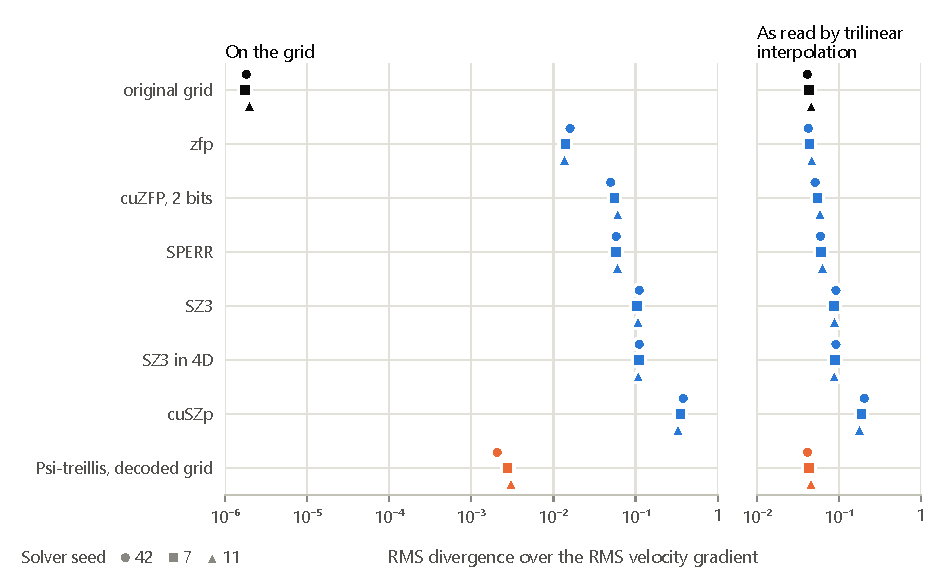
\includegraphics[width=\linewidth]{figures/divergence}
  \caption{Divergence of one frame as each chain gives it back, relative to the RMS velocity gradient, on three
  realisations at $256^3$ (one marker each, stacked within a row). Left: on the grid, by spectral differentiation. Right: as read by
  trilinear interpolation. The compressors receive a bound of 5\,\% of $\urms$; cuZFP is at a fixed rate of 2 bits per
  value. For \codec\ the grid is the one its library decodes; the field it actually reads, the curl of the potential,
  has a divergence of \val{div.psi.max} (not shown).}
  \label{fig:divergence}
\end{figure}

\begin{table}[t]
  \centering
  % Written by tools/paper_numbers.py from the logs of benchmarks/. Do not edit: run the script again.
\begin{tabular}{lrrrr}
\toprule
 & Compression & RMS error & Divergence & Divergence \\
Chain & ratio & (\%) & on the grid (\%) & as read (\%) \\
\midrule
original grid &  &  & $<$0.0002 & 4.1 to 4.6 \\
zfp & 11 & 0.15 & 1.4 to 1.6 & 4.3 to 4.7 \\
cuZFP, 2 bits & 16 & 0.46 & 5.0 to 6.1 & 5.2 to 5.9 \\
SPERR & 110 & 0.83 & 5.8 to 6.0 & 6.0 to 6.3 \\
SZ3 & 147 & 1.79 & 10.4 to 11.1 & 8.7 to 9.2 \\
SZ3 in 4D & 337 & 1.79 & 10.8 to 11.1 & 8.8 to 9.2 \\
cuSZp & 12 & 2.89 & 32.8 to 38.0 & 17.9 to 20.5 \\
\codec, decoded grid & 134 & 0.62 & 0.2 to 0.3 & 4.2 to 4.6 \\
\bottomrule
\end{tabular}

  \caption{The figures of figure~\ref{fig:divergence}: range over the three realisations. The compression ratio and the
  relative RMS error are those of the realisation of seed 42; for SZ3 in 4D and \codec\ the ratio is that of a block
  of 32 frames.}
  \label{tab:divergence}
\end{table}

Three facts follow.
\begin{itemize}
  \item \textbf{Compression alone breaks the law.} The original grids have a spectral divergence of at most
  \val{grid.raw.max} of the gradient, the rounding of single precision. After SZ3 it is \val{grid.sz3.min} to
  \val{grid.sz3.max}\,\%, after SZ3 in 4D \val{grid.sz3_4d.min} to \val{grid.sz3_4d.max}\,\%, after SPERR
  \val{grid.sperr.min} to \val{grid.sperr.max}\,\%. A bound on each value does not bound a derivative.
  \item \textbf{Reading alone breaks it too.} The trilinear interpolant of the \emph{original} grid has a divergence of
  \val{read.raw.min} to \val{read.raw.max}\,\% of the gradient: its derivative along an axis is piecewise constant
  along that axis, so the three terms of the divergence no longer cancel.
  \item \textbf{Compression adds to it.} Read by the same interpolation, the grids decoded by SZ3 have
  \val{read.sz3.ratio.min} to \val{read.sz3.ratio.max} times the divergence of the original grid, those decoded by
  SPERR \val{read.sperr.ratio.min} to \val{read.sperr.ratio.max} times.
\end{itemize}
The grid decoded by \codec\ carries a spectral divergence of \val{grid.psi.min} to \val{grid.psi.max}\,\%: it is a
sampling of a solenoidal field at voxel centres, which is not a solenoidal grid. And if that grid is read by trilinear
interpolation, its divergence is that of the original grid (\val{read.psi.min} to \val{read.psi.max}\,\%). The benefit of
the representation therefore exists only when its field is read directly, as section~\ref{sec:method} describes, and
not when it is decoded to a grid.

\subsection{What it does to tracers}

Table~\ref{tab:tracers} gives the two tracer measurements on the realisation of seed 42, with 8 tracers per voxel.
The criterion fixed in advance for the original grid and for cuZFP was more than 5 standard errors of clustering; for
\codec, less than 2 in absolute value. The grids decoded by SZ3 and SPERR had no clustering criterion: we did not know
where they would fall.

\begin{table}[t]
  \centering
  % Written by tools/paper_numbers.py from the logs of benchmarks/. Do not edit: run the script again.
\begin{tabular}{lrrr}
\toprule
 & Clustering & Growth of var($D$) & Relative to the \\
Chain & (standard errors) & per Kolmogorov time & original grid \\
\midrule
original grid & 3.2 & $9.0\times10^{-5}$ & 1 \\
cuZFP, 2 bits & 32.8 & $2.5\times10^{-4}$ & 2.8 \\
SPERR & 107 & $6.3\times10^{-4}$ & 7.0 \\
SZ3 & 672 & $2.4\times10^{-3}$ & 26 \\
SZ3 in 4D & 720 & $2.4\times10^{-3}$ & 26 \\
\codec, bound 5\,\% & 0.4 & $1.9\times10^{-8}$ & 1/4,729 \\
\bottomrule
\end{tabular}

  \caption{Tracers advected in one frozen $256^3$ frame seen through each chain, 10 Kolmogorov times, tracer seeds 1
  to 5. Clustering: excess dispersion of the count per bin of one voxel, in standard errors. Growth of the variance of
  $D$, the logarithm of the volume carried by a tracer, per Kolmogorov time, and relative to the original grid.
  Every grid is read as a half-precision texture with hardware trilinear filtering.}
  \label{tab:tracers}
\end{table}

\begin{figure}[t]
  \centering
  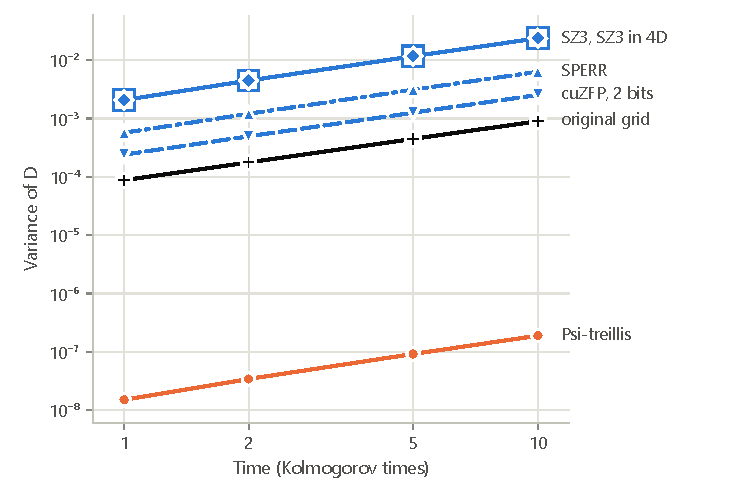
\includegraphics[width=0.78\linewidth]{figures/tracers}
  \caption{Variance of $D$, the logarithm of the volume carried by a tracer, against time in Kolmogorov times, for the
  chains of table~\ref{tab:tracers}; the curves of SZ3 and of SZ3 in 4D coincide. For \codec\ the value is the truncation error of the centred differences used to
  measure the divergence, not a divergence of its field.}
  \label{fig:tracers}
\end{figure}

Through the grids decoded by SZ3 and by SPERR, the tracers cluster by \val{trac.sz3.z} and \val{trac.sperr.z} standard
errors, and the variance of the volume they carry grows \val{trac.sz3.over.raw} and \val{trac.sperr.over.raw} times
faster than through the original grid. Through cuZFP at 2 bits per value they cluster by \val{trac.zfp2.z} standard
errors. Through \codec\ with the same 5\,\% bound, the excess is \val{trac.psi3b.z} standard errors and the variance
grows \val{trac.raw.over.psi} times more slowly than through the original grid.

One result goes against what we expected. The trilinear texture of the \emph{uncompressed} frame does not pass the
clustering threshold fixed in advance: \val{trac.raw.z} standard errors here, \val{lagr.256.tex.z} and
\val{lagr.512.tex.z} on the two sequences of the first campaign, \val{lagr.conf.tex.z} on another realisation, for a
threshold of 5. On resolved data, this clustering test does not separate \codec\ from plain trilinear interpolation;
only the drift of the volume does (figure~\ref{fig:tracers}). After 100 Kolmogorov times, measured on one seed, the
standard deviation of $D$ is \val{long.zfp2.std} through cuZFP, \val{long.tex.std} through the trilinear texture,
\val{long.cubic.std} through tricubic interpolation and \val{long.psi3.std} through \codec.

\subsection{What a replayed frame costs}

Table~\ref{tab:playback} gives the cost of one frame when a sequence is replayed with 4 million particles: the data
read from disk, the GPU memory held and the time, each measured by the same program during one run per case.

\begin{table}[t]
  \centering
  % Written by tools/paper_numbers.py from the logs of benchmarks/. Do not edit: run the script again.
\begin{tabular}{llrrrrrr}
\toprule
 & & Read & GPU memory & Disk & Decoding & RK4 step & Frame \\
Grid & Chain & (MiB) & (MiB) & (ms) & (ms) & (ms) & (ms) \\
\midrule
$256^3$ & cuZFP, 2 bits & 12.00 & 590 & 2.39 & 1.05 & 0.53 & 5.3 \\
$256^3$ & \codec & 1.38 & 192 & 0.30 & 0.73 & 6.46 & 14.2 \\
\addlinespace
$256^3$ & raw frames & 192.00 & 576 & 41.19 & 0.51 & 0.49 & 50.2 \\
$256^3$ & \codec & 1.38 & 192 & 0.30 & 0.70 & 5.98 & 13.2 \\
\addlinespace
$512^3$ & cuZFP, 2 bits & 96.00 & 3810 & 43.96 & 7.68 & 1.87 & 59.3 \\
$512^3$ & \codec & 10.53 & 624 & 3.81 & 3.43 & 6.96 & 21.7 \\
\addlinespace
$512^3$ & raw frames & 1536.00 & 3712 & 871.57 & 5.92 & 2.74 & 941.9 \\
$512^3$ & \codec & 10.53 & 624 & 3.60 & 4.75 & 9.18 & 27.4 \\
\bottomrule
\end{tabular}

  \caption{Cost of one replayed frame, 4 million sorted particles, two Runge--Kutta steps per frame. Each line is one
  side of a run that compares two chains on the same frames. The time of a frame is the sum of disk, bus, decoding,
  sort and advection times. \codec\ is of degree 3 without a bound; cuZFP is at 2 bits per value.}
  \label{tab:playback}
\end{table}

Against raw frames at $512^3$, \codec\ reads \val{play.512.raw.over.psi.read} times less data and holds
\val{play.512.raw.over.psi.mem} times less GPU memory, and the frame costs \val{play.512.raw.over.psi.time} times less,
the raw chain being dominated by the reading of 1.5\,GiB per frame. Against cuZFP the result depends on the size. At $256^3$ it goes against \codec: it reads
\val{play.256.zfp.over.psi.read} times less data and holds \val{play.256.zfp.over.psi.mem} times less memory, but its
frame costs \val{play.256.psi.time}\,ms against \val{play.256.zfp.time}\,ms, because one Runge--Kutta step costs
\val{play.256.psi.rk4}\,ms through the lattice against \val{play.256.zfp.rk4}\,ms through the texture. We attribute
this to the cost of evaluating 64 spline nodes per sample, against one trilinear fetch in a texture that fits in the
cache; we did not isolate it. At $512^3$ the step through the lattice is still the slower one
(\val{play.512.psi.rk4}\,ms against \val{play.512.zfp.rk4}\,ms), but the frame of \codec\ costs
\val{play.512.psi.time}\,ms against \val{play.512.zfp.time}\,ms: the cuZFP chain then spends
\val{play.512.zfp.disk}\,ms reading \val{play.512.zfp.read}\,MiB per frame from disk. These times are those of one
run each, in which the two chains share the GPU: next to the raw chain, the same \codec\ file costs
\val{play.512.psi.time.raw}\,ms per frame instead of \val{play.512.psi.time}\,ms. The speed of sampling is therefore not
an argument for the method; the data read and the memory held are.

\section{Method}
\label{sec:method}

\subsection{Representation}

A frame is a velocity field $\mathbf{u}$ on a periodic cubic grid of $n^3$ voxels, $n$ a power of two. \codec\ writes it
\begin{equation}
  \mathbf{u}(\mathbf{x}) = \overline{\mathbf{u}} + \nabla \times \boldsymbol{\Psi}(\mathbf{x}), \qquad
  \boldsymbol{\Psi}(\mathbf{x}) = \delta \sum_{\mathbf{j}} \mathbf{q}_{\mathbf{j}}\,
  B^{d}\!\left(\tfrac{\mathbf{x}}{h} - \mathbf{j}\right),
  \label{eq:representation}
\end{equation}
where $\overline{\mathbf{u}}$ is the mean velocity of the frame, $B^{d}$ is the tensor-product cardinal B-spline of
degree $d = 2$ or $3$~\cite{unser1999splines}, the nodes $\mathbf{j}$ form a periodic lattice of step $h$ (2 voxels by
default), the coefficients $\mathbf{q}_{\mathbf{j}}$ are vectors of three integers and $\delta$ is a quantisation step.
Since $\nabla\cdot(\nabla\times\boldsymbol{\Psi}) = 0$ identically, the field of equation~\eqref{eq:representation}
has zero divergence at every point, whatever the integers: quantisation and every later approximation act on
$\boldsymbol{\Psi}$, and cannot create a divergence. The price is that the compressible part of the input, if it has
one, is lost.

Figure~\ref{fig:chains} sets this chain against the usual one. The velocity at a point is the analytic curl of the splines. It depends on the $(d+1)^3$ nodes around the point, 27
in degree 2 and 64 in degree 3, and is evaluated directly from the integers: no grid of velocities is rebuilt.

\begin{figure}[t]
  \centering
  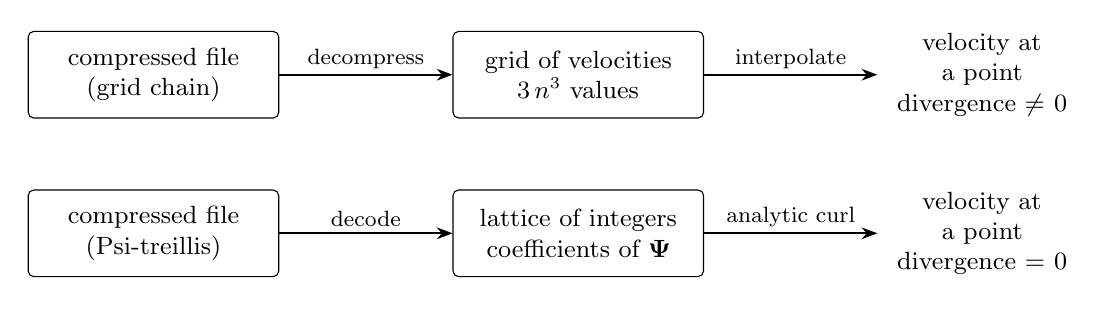
\begin{tikzpicture}[
      font=\small, node distance=4mm and 22mm,
      box/.style={draw, rounded corners=2pt, align=center, inner sep=4pt, minimum height=11mm, text width=29mm},
      result/.style={align=center, inner sep=2pt, text width=25mm},
      arr/.style={-{Stealth[length=2mm]}, semithick},
      lab/.style={font=\footnotesize, midway, above, inner sep=2pt}]
    \node[box] (fa) {compressed file\\(grid chain)};
    \node[box, right=of fa] (ga) {grid of velocities\\$3\,n^3$ values};
    \node[result, right=of ga] (ua) {velocity at a point\\divergence $\neq 0$};
    \draw[arr] (fa) -- node[lab] {decompress} (ga);
    \draw[arr] (ga) -- node[lab] {interpolate} (ua);
    \node[box, below=9mm of fa] (fb) {compressed file\\(\codec)};
    \node[box, right=of fb] (gb) {lattice of integers\\coefficients of $\boldsymbol{\Psi}$};
    \node[result, right=of gb] (ub) {velocity at a point\\divergence $= 0$};
    \draw[arr] (fb) -- node[lab] {decode} (gb);
    \draw[arr] (gb) -- node[lab] {analytic curl} (ub);
  \end{tikzpicture}
  \caption{The two chains compared. In the usual chain, a frame is decompressed to a grid of velocities and the
  velocity at a point is interpolated from it. \codec\ decodes a lattice of integer coefficients of the vector
  potential, on a lattice of step 2 voxels, and evaluates its analytic curl at the point: no grid of velocities is
  rebuilt, and the divergence is zero by identity.}
  \label{fig:chains}
\end{figure}

\subsection{Encoding}

\paragraph{Projection.}
The encoder takes the periodic Fourier transform of the frame and fits the potential in Fourier space, one lattice wave
vector at a time: it sums over the wave vectors of the data that alias onto it and solves a $3\times3$ normal system,
regularised by a small ridge term (the potential is defined only up to a gradient). The coefficients are organised as
a pyramid of three nested lattices, each twice as coarse as the previous one. The coarsest level is fitted and
quantised first; each finer level fits what the coarser levels, as decoded, leave. The quantisation step is set from a
target RMS error given as a fraction of the RMS velocity $\urms$ (0.5\,\% by default). The coefficients of the finest
level fit in 8 bits, those of the other levels in 16.

\paragraph{Temporal prediction.}
A frame is predicted from the two previous ones and a Laplacian term,
\begin{equation}
  \hat{q}^{\,k+1} = \left\lfloor \frac{a\,q^{k} + b\,q^{k-1} + c\,\Delta q^{k} + 512}{1024} \right\rfloor ,
\end{equation}
with three integers $(a, b, c)$ per level, fitted once per file on a few frames, and $\Delta$ the six-neighbour
Laplacian on the lattice. Encoder and reader compute this prediction with the same integer arithmetic, so that the
reader reproduces the state of the encoder exactly. The difference between a coefficient and its prediction, the
innovation, is coded on 8 bits; the rare values that do not fit are listed apart. One frame in 32 is a key frame,
decodable on its own, coded with a three-dimensional Lorenzo predictor.

\paragraph{Entropy coding.}
Innovations and key frames are coded with a range variant of asymmetric numeral systems
(rANS)~\cite{duda2013asymmetric}, in independent blocks of 1024 symbols, so that the GPU decodes all the blocks of a
frame in parallel.

\paragraph{Sampling lattice.}
The reader does not sample the pyramid. From the three decoded levels it builds one lattice at the step of the finest
level by the exact two-scale relation of the B-splines, in integer arithmetic, and keeps it in GPU memory for two
consecutive frames. This lattice of integers is what the sampling kernels read.

\subsection{Verified bound on the largest error}

The lattice of step 2 voxels cannot follow the field everywhere. When a tolerance is given, the encoder adds a second
potential of step 1 voxel, stored sparsely by bricks of $4^3$ nodes with 8-bit coefficients, only where the first one
leaves an error above the tolerance. Because the correction is itself the curl of a potential, the corrected field
stays divergence-free; a correction applied to the velocity values would not.

The encoder then decodes each frame as the reader will, with the arithmetic of the reader, and measures the largest
error of a velocity component over all the voxels of all the frames. It reports whether that error is below the
tolerance minus half of a margin of $10^{-4}\,\urms$, kept for the rounding differences between two GPU kernels. If the bound
is not held, or if holding it would require refining more than a quarter of the volume, the encoder says so and
returns an error code: a file is never presented as bounded when it is not. The bound is therefore verified, not
proved: it holds at voxel centres and at the instants of the frames, for the file as written, and the margin is
empirical.

\subsection{Reading}

A file holds a header, the frames, a table that locates them, and a seal. The reader decodes a frame on the GPU (rANS,
prediction, synthesis of the sampling lattice) and compares a 64-bit fingerprint of the decoded state with the one the
encoder stored in the table: a frame whose state differs is reported. The public interface is a C library with a
command-line tool and a Python module; it compresses a sequence, decodes a frame to the grid, and samples the velocity
at arbitrary points. The file format is specified in \texttt{docs/FORMAT.md}, and two readers were written from that
specification alone to test it (section~\ref{sec:reproducibility}).

\section{Results}
\label{sec:results}

\subsection{Compression, bound and speed}

On 55 frames of the $512^3$ sequence, with degree 3 and the default settings, \codec\ compresses
\val{comp.512.d3.ratio} times for a relative RMS field error of \val{comp.512.d3.rms}\,\%; in degree 2,
\val{comp.512.d2.ratio} times for \val{comp.512.d2.rms}\,\%. With a bound of 5, 4 and 3\,\% of $\urms$ on the largest
error, verified on every voxel of every frame, the compression ratio in degree 3 is \val{comp.512.d3.t05.ratio},
\val{comp.512.d3.t04.ratio} and \val{comp.512.d3.t03.ratio}; at $256^3$ it is \val{comp.256.d3.t05.ratio},
\val{comp.256.d3.t04.ratio} and \val{comp.256.d3.t03.ratio}. The six files hold their bound. These ratios are those of
a file with a key frame every 32 frames: they include the gain of temporal prediction.

The bound has a floor. In degree 2 it is held at 6\,\% at $256^3$ and at 7\,\% at $512^3$ but missed one point lower,
on one frame in each case: once all the nodes of the fine level around a voxel are retained, nothing more can be added.

Read back, the twelve reference files of the repository (the ten files with a bound above, and the two files without
a bound at $512^3$) give the state the encoder recorded for every frame, and the ten files with a bound give the same
field at \val{readback.points} points off the grid. Through the public interface and a different code path, the field decoded
to the grid at $512^3$ and compared with the raw frames in NumPy has the error the encoder recorded, and it is within
the tolerance of each file whose bound is held.

On the machine of this study, at $512^3$ and in degree 3, a frame is decoded in \val{speed.z.decode}\,ms and one
Runge--Kutta step of 4 million sorted particles takes \val{speed.z.rk4}\,ms (medians of \val{speed.repetitions}
repetitions); with the 5\,\% bound, \val{speed.f.decode}\,ms and \val{speed.f.rk4}\,ms. Encoding takes
\val{enc.512.t05}\,ms per frame with the 5\,\% bound and \val{enc.512.t03}\,ms with the 3\,\% bound, in one run each.
These timings are those of the reader running alone, and are not claimed for another machine. In the visual comparator
of table~\ref{tab:playback}, where two chains run on the same GPU, the same step takes \val{play.512.psi.rk4}\,ms; we
did not isolate the cause of the difference.

The energy spectrum of the decoded grid stays close to that of the original: without a bound, on the three
realisations at $256^3$, the enstrophy is within \val{spec.psi.enstrophy.max}\,\% of the original, and the spectrum
departs from it by more than 10\,\% only from wavenumber \val{spec.psi.k10.min} to \val{spec.psi.k10.max}, for a
truncation of the solver at \val{spec.truncation}.

\subsection{The price: compression at an equal bound}

Table~\ref{tab:equal} and figure~\ref{fig:equal} compare \codec\ with the other compressors when all receive the same
bound on the largest error, on the same 32 frames, every error being measured in the same way.

\begin{table}[t]
  \centering
  \small\setlength{\tabcolsep}{4pt}
  % Written by tools/paper_numbers.py from the logs of benchmarks/. Do not edit: run the script again.
\begin{tabular}{llrrrrrr}
\toprule
Grid & Bound & \codec & SZ3 in 4D & SZ3 & SPERR & cuSZp & zfp \\
\midrule
$256^3$ & 5\,\% & 133.7 / 0.614 & 334.0 / 1.690 & 148.1 / 1.776 & 109.2 / 0.831 & 11.9 / 2.869 & 11.5 / 0.146 \\
$256^3$ & 4\,\% & 126.7 / 0.604 & 267.8 / 1.391 & 118.3 / 1.466 & 93.6 / 0.709 & 11.1 / 2.296 & 9.1 / 0.079 \\
$256^3$ & 3\,\% & 104.0 / 0.582 & 201.6 / 1.086 & 90.3 / 1.145 & 76.9 / 0.578 & 10.1 / 1.722 & 9.1 / 0.079 \\
$256^3$ & 1.5\,\% & not encoded & 106.1 / 0.602 & 49.5 / 0.638 & 48.8 / 0.346 & 8.2 / 0.861 & 7.4 / 0.042 \\
\addlinespace
$512^3$ & 5\,\% & 137.6 / 0.623 & 225.2 / 1.778 & 167.4 / 1.754 & 117.1 / 0.818 & 12.5 / 2.886 & 11.4 / 0.136 \\
$512^3$ & 4\,\% & 127.4 / 0.609 & 179.5 / 1.464 & 134.0 / 1.447 & 100.0 / 0.700 & 11.7 / 2.309 & 11.4 / 0.136 \\
$512^3$ & 3\,\% & 100.6 / 0.582 & 134.1 / 1.142 & 101.3 / 1.131 & 81.8 / 0.571 & 10.7 / 1.732 & 9.0 / 0.073 \\
\bottomrule
\end{tabular}

  \caption{Compression ratio and relative RMS error at an equal bound on the largest error, on 32 frames: frames 16
  to 47 of the $256^3$ sequence, frames 0 to 31 of the $512^3$ sequence. \codec\ encodes the 32 frames as one group;
  SZ3 in 4D takes them as one block at $256^3$ and as four blocks of 8 frames at $512^3$, where a block of 32 does not
  fit in the memory of the machine; the other compressors work frame by frame.}
  \label{tab:equal}
\end{table}

\begin{figure}[t]
  \centering
  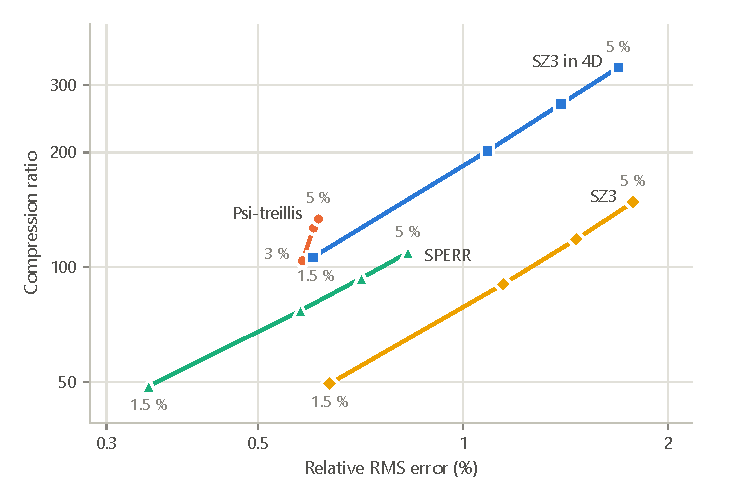
\includegraphics[width=0.78\linewidth]{figures/equal_bound}
  \caption{Compression ratio against relative RMS error at $256^3$, for bounds of 5, 4, 3 and 1.5\,\% of $\urms$ on the
  largest error (from right to left on each curve). \codec\ could not be encoded at 1.5\,\%. cuSZp and zfp, near a
  ratio of 10, are not drawn. Up and to the left is better.}
  \label{fig:equal}
\end{figure}

\begin{itemize}
  \item \textbf{At an equal bound, SZ3 in 4D compresses \val{eq.256.sz4d.over.psi.min} to
  \val{eq.256.sz4d.over.psi.max} times more} than \codec\ at $256^3$, with an RMS error
  \val{eq.256.sz4d.rms.over.psi.min} to \val{eq.256.sz4d.rms.over.psi.max} times larger. This claim of ours, that
  \codec\ would compress at least as much, does not hold.
  \item \textbf{Against SPERR, \codec\ compresses \val{eq.sperr.under.psi.min} to \val{eq.sperr.under.psi.max} times
  more} over the five cases measured, with an RMS error that is lower or equal within 1\,\%. \codec\ uses the time
  direction; SPERR is applied frame by frame.
  \item \textbf{At an equal RMS error the order is reversed, in a narrow window.} The three points of \codec\ at
  $256^3$ are not dominated by any of the \val{eq.256.other.points} points of the other compressors: for an RMS error of
  \val{eq.256.sz4d.t015.rms}\,\%, SZ3 in 4D needs a bound of 1.5\,\% and compresses \val{eq.256.sz4d.t015.ratio} times,
  where \codec\ compresses \val{eq.256.psi.t05.ratio} times at \val{eq.256.psi.t05.rms}\,\%. But \codec\ has only that
  window, an RMS error of \val{eq.256.psi.rms.min} to \val{eq.256.psi.rms.max}\,\%; the other compressors trade ratio for
  error over a wide range, and it does not.
  \item zfp is not at an equal attained bound: its fixed-accuracy mode leaves the largest error at
  \val{eq.256.zfp.t05.max}\,\% of $\urms$ for a bound of 5\,\%. It is listed for the record.
\end{itemize}

\subsection{Where it works: the resolution of the data}
\label{sec:validity}

The lattice has a step of 2 voxels. Whether it can follow the field depends on how the smallest scales of the flow
compare with that step. Eighteen sequences at $256^3$, six viscosities and three solver seeds each, span a Kolmogorov
scale of \val{valid.eta.min} to \val{valid.eta.max} voxel (figure~\ref{fig:validity}). The criteria of this sweep
were written before its first measurement.

\begin{figure}[t]
  \centering
  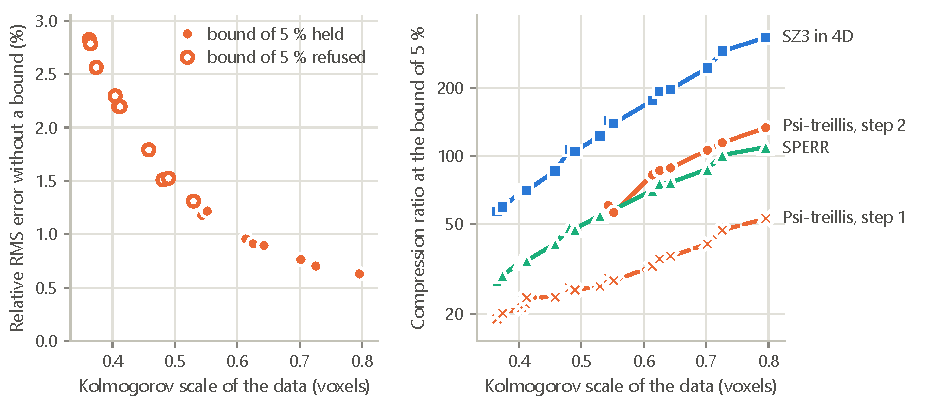
\includegraphics[width=\linewidth]{figures/validity}
  \caption{Resolution sweep, 18 sequences at $256^3$. Left: relative RMS error of \codec\ without a bound against the
  Kolmogorov scale of the data, one marker per sequence; filled markers are the sequences on which a bound of 5\,\% of
  $\urms$ could be held at the default lattice step. Right: compression ratio at that bound for \codec\ at lattice steps of 2 and 1 voxels,
  SPERR and SZ3 in 4D.}
  \label{fig:validity}
\end{figure}

\begin{itemize}
  \item \textbf{The bound needs resolved data.} At the default step, the 5\,\% bound is held on the
  \val{valid.held} sequences whose Kolmogorov scale is \val{valid.eta.held.min} voxel or more, and refused on the
  \val{valid.refused} below (\val{valid.eta.refused.max} voxel or less); the threshold is at \val{valid.eta.star}
  voxel. The 3\,\% bound is held only on the \val{valid.held.t03} sequences at \val{valid.eta.held.t03.min} voxel or
  more. Without a bound, the RMS error grows from \val{valid.rms.best}\,\% to \val{valid.rms.worst}\,\% as the
  resolution decreases.
  \item \textbf{Near the threshold, SPERR compresses more.} \codec\ is ahead of SPERR on \val{valid.ahead} of the
  \val{valid.held} sequences where its bound holds, by up to \val{valid.sperr.best} times, and behind on the others
  (\val{valid.sperr.worst} times its ratio at worst): there the bound is held at the price of a fine level that costs
  a large part of the file. Our claim that it would be ahead wherever the bound holds does not hold.
  \item \textbf{A lattice step of 1 voxel holds the bound everywhere}, on the 18 sequences, but at
  \val{valid.mf1.sperr.min} to \val{valid.mf1.sperr.max} times the compression ratio of SPERR.
  \item \textbf{One sequence per setting is not enough.} Between the three realisations of one viscosity, the
  compression ratio varies by up to \val{valid.spread.ratio}\,\% and the RMS error by up to
  \val{valid.spread.rms}\,\%. Part of this is a spread of resolution: the Kolmogorov scale itself differs between
  realisations.
\end{itemize}

The same degradation is seen at $512^3$ on a sequence at \val{reso.eta} voxel per Kolmogorov scale: \val{reso.ratio}
times for an RMS error of \val{reso.rms}\,\%, and the bound refused at 5, 4 and 3\,\%.

\section{Limits}
\label{sec:limits}

\paragraph{No public dataset.}
Every result of this article comes from our own solver. We obtained access to the Johns Hopkins Turbulence
Databases~\cite{li2008public,jhtdbisotropic} to measure a cutout of their forced isotropic dataset at $1024^3$, but no complete frame
could be retrieved: the transfers of the cutout broke repeatedly. To fill this gap as far as we could, we simulated a
turbulence as poorly resolved as that dataset (\val{reso.eta} voxel per Kolmogorov scale, against 0.46 to 0.47 for
the database, computed from the Kolmogorov length and the grid it documents), we swept the resolution over 18
sequences, and we validated on our own data a protocol that measures the codec on a windowed, non-periodic cutout
(the error at the centre of the cutout is \val{ctrl.ratio.min} to \val{ctrl.ratio.max} times that of the whole
field). These measurements predict that the method would degrade on that dataset, whose resolution is below the
threshold of section~\ref{sec:validity}. They do not replace the trial: nothing shows that data from another solver
behave as ours do. The scripts of the trial and its criteria, written in advance, are in the repository.

\paragraph{One machine, one family of flows.}
Everything is measured on one GPU under Windows, on periodic isotropic turbulence at $256^3$ and $512^3$. The
library is compiled on Linux by a workflow of the repository, on a machine without a GPU; it has not been run there, apart from the CPU reference reader. By our estimate of its memory needs (about 31\,GiB), the encoder
does not handle $1024^3$ on a GPU of 24\,GiB. Nothing is established for flows with walls, for non-periodic domains, or for fields
that are not solenoidal, whose compressible part the representation discards.

\paragraph{The bound.}
It is verified, not proved: it holds at voxel centres and at the instants of the frames, and its arithmetic margin is
empirical. Below \val{valid.eta.star} voxel per Kolmogorov scale it cannot be held at the default lattice step.

\paragraph{Compression and speed.}
At an equal bound \codec\ compresses less than SZ3 in 4D everywhere, and less than SPERR near the resolution
threshold. Its sampling is slower than that of a texture, and at $256^3$ its frame costs more time than that of cuZFP. The compressors it is
compared with run with their default settings; a specialist might obtain more from them.

\paragraph{The comparison of tracers.}
The tracer experiment uses a frozen frame, tracers without inertia, and one frame per sequence. The clustering test
fixed in advance does not separate \codec\ from trilinear interpolation of the uncompressed field. A confirmation of
the first campaign on another realisation, with every parameter fixed in advance, met three of its four conditions;
the fourth failed on one path, a reference lattice of step 1 voxel, at \val{lagr.conf.ref.z} standard errors for a
threshold of 2 in absolute value (\val{lagr.conf.ref.z.ten} on ten seeds, run afterwards). As registered, that
confirmation does not hold.

\paragraph{The format.}
The specification was sufficient for two independent readers to decode every frame, but the writing of the
second brought out six passages where the text left a doubt, one of which concerns the decoded state; they have since been
completed, and no reader has yet been written from the completed text. One of them is a limit of the format: nothing
bounds the coefficients of the temporal predictor, so that a file written on purpose could overflow the 32-bit sum of
the prediction. In the files read by the second reader, the predictors are at least \val{ref.py.margin} times below that limit. The reader does not see every alteration of a file
without a seal.

\paragraph{Prior work.}
Our statement that no earlier work stores a quantised, entropy-coded vector potential rests on web searches. We
could not read the full text of~\cite{ravu2016creating}, only its abstract. For several of the works cited, only the
bibliographic record and the title or the project page were read; \texttt{paper/references\_verification.md} says which.

\section{Reproducibility}
\label{sec:reproducibility}

The repository (\url{https://github.com/Pluenet-Killian/Psi-treillis}) holds the codec, its tests, and every
measurement of this article with the script that produces it.
\begin{itemize}
  \item \textbf{Claims.} \texttt{docs/CLAIMS.md} lists \val{claims.total} claims: statement, numerical criterion,
  measured value, command that reproduces the measurement, verdict. \val{claims.hold} hold, \val{claims.fail} do not,
  and \val{claims.pending} are hypotheses not yet tested (appendix). \texttt{python tools/claims.py} recomputes every
  verdict from the logs kept in \texttt{benchmarks/}, without a GPU.
  \item \textbf{No number typed by hand.} Every number of this article is read from those logs by
  \texttt{tools/paper\_numbers.py}, which writes the file of values and the tables the text includes.
  \item \textbf{One code.} All the logs were produced by the code of the repository as published, after the sources
  were reorganised; the compression ratios and the errors are deterministic and can be compared digit for digit, the
  timings cannot.
  \item \textbf{Tests.} With the same options the encoder writes the same bytes. A suite of \val{test.cases} cases
  checks the fingerprints of the files written, the bound, the read-back and the refusal of altered files; another
  checks the public interface.
  \item \textbf{Two independent readers.} A C++ reader and a Python reader were each written from the specification of
  the format, without reading the code of the codec. They recompute the fingerprint of every frame they read
  (\val{ref.cpp.frames} frames of twelve files for the first, \val{ref.py.frames} frames of \val{ref.py.files} files
  for the second) and give the velocity at the probe points within \val{ref.cpp.field} and \val{ref.py.field} of
  $\urms$ of the field of the encoder.
  \item \textbf{Data.} The sequences are not distributed (9 to 96\,GiB each); the solver regenerates them with the
  commands given in the repository.
\end{itemize}

\section{Conclusion}

Storing the vector potential of an incompressible flow on a B-spline lattice gives a compressed field that has zero
divergence at every point and that a GPU samples without rebuilding a grid of velocities. On resolved periodic
turbulence, the measurements confirm what this buys: tracers advected through it do not cluster and the volume they
carry does not drift, where they cluster strongly through the same frames decoded by SZ3 or SPERR at the same bound;
and a replayed frame reads and holds several times less data than a decoded texture. They also fix its price and its
domain: at an equal bound it compresses \val{eq.256.sz4d.over.psi.min} to \val{eq.256.sz4d.over.psi.max} times less
than the best of the compressors we tested, its sampling is slower than that of a texture, and its bound cannot be held on
data whose
Kolmogorov scale is below \val{valid.eta.star} voxel.

Three things would change what can be said: a measurement on a public dataset; a second machine; and a lattice
whose step adapts to the flow, which the validity map suggests and which we have not tried.

{\small\sloppy
\bibliographystyle{unsrtnat}
\bibliography{references}
}

\appendix
\section{The claims}
\label{sec:claims}

Table~\ref{tab:claims} lists the claims of \texttt{docs/CLAIMS.md} with their verdicts. A claim that does not hold is
something the project would have liked to assert and that its own measurements refute.

{\small
% Written by tools/paper_numbers.py from the logs of benchmarks/. Do not edit: run the script again.
\begin{longtable}{@{}lp{10.6cm}l@{}}
\caption{The claims of the project and their verdicts.\label{tab:claims}}\\
\toprule
Identifier & Claim & Verdict \\
\midrule
\endfirsthead
\toprule
Identifier & Claim & Verdict \\
\midrule
\endhead
\bottomrule
\endfoot
COMP-1 & Compression without a bound, degree 3 & holds \\
COMP-2 & Compression without a bound, degree 2 & holds \\
BOUND-1 & Certified bound, degree 3 & holds \\
BOUND-2 & Cost of the bound, degree 3 & holds \\
BOUND-3 & Certified bound, degree 2 & holds \\
READBACK-1 & Read-back consistent with the encoding & holds \\
DIV-1 & Zero divergence & holds \\
SPEED-1 & Reading speed & holds \\
ENC-1 & Encoding speed & holds \\
LAGR-1 & Clustering of tracers under cuZFP & holds \\
LAGR-2 & No clustering under Psi-treillis & holds \\
LAGR-3 & Volume carried by a tracer & holds \\
ROBUST-1 & Reader faced with an altered file & holds \\
TEST-1 & Determinism and non-regression & holds \\
API-1 & Public interface, round trip at 64$^3$ & holds \\
API-2 & Errors read back at 512$^3$ through another code path & holds \\
BENCH-1 & Against SPERR, at an equal bound & holds \\
BENCH-2 & Pareto front at 256$^3$ & holds \\
REF-1 & A reader independent of the code & holds \\
LAGR-4 & Clustering under the trilinear texture & \textbf{does not hold} \\
BOUND-4 & Certified bound, degree 2, one point lower & \textbf{does not hold} \\
RESO-1 & Fidelity on a less resolved turbulence & \textbf{does not hold} \\
RESO-2 & Certified bound on a less resolved turbulence & \textbf{does not hold} \\
BENCH-3 & Against SZ3 in 4D, at an equal bound & \textbf{does not hold} \\
JHTDB-1 & Expected degradation on JHTDB & \textbf{pending} \\
JHTDB-2 & Usefulness for compression on JHTDB & \textbf{pending} \\
PORT-1 & Another machine & \textbf{pending} \\
LAGR-5 & Lagrangian confirmation on an independent realisation & \textbf{does not hold} \\
BENCH-4 & SZ3 in 4D on 32 frames at 512$^3$ & \textbf{pending} \\
VALID-1 & Resolution threshold of the bound of 5 \% & holds \\
VALID-2 & Ahead of SPERR where the bound holds & \textbf{does not hold} \\
VALID-3 & The step of 1 voxel holds the bound everywhere, without catching up on the compression ratio & holds \\
VALID-4 & Field error as a function of the resolution & \textbf{does not hold} \\
VALID-5 & Spread between realisations & \textbf{does not hold} \\
CTRL-1 & Windowed cutout protocol & holds \\
JHTDB-3 & Degradation on a JHTDB cutout & \textbf{pending} \\
JHTDB-4 & Step of 1 voxel on the JHTDB cutout & \textbf{pending} \\
REPR-1 & Does our under-resolved sequence stand in for JHTDB? & \textbf{pending} \\
REF-2 & A second reader from the completed specification & \textbf{does not hold} \\
LINUX-1 & Compilation under Linux & \textbf{pending} \\
GRID-1 & Compression alone breaks the law & holds \\
READ-1 & Reading alone breaks the law & holds \\
READ-2 & Compression adds to it & holds \\
TRAC-1 & Tracers after an error-bounded compressor & holds \\
SPEC-1 & Spectrum of Psi-treillis & holds \\
PLAY-1 & Cost of one replayed frame & holds \\
REF-3 & A third reader from the specification completed on 17 November 2026 & \textbf{pending} \\
\end{longtable}

}

\end{document}
